\documentclass[11pt, a4paper, twoside]{article}   	% use "amsart" instead of "article" for AMSLaTeX format

\usepackage{geometry}                		% See geometry.pdf to learn the layout options. There are lots.
\usepackage{pdfpages}
\usepackage{caption}
\usepackage{minted}
\usepackage[german]{babel}			% this end the next are needed for german umlaute
\usepackage[utf8]{inputenc}
\usepackage{color}
\usepackage{graphicx}
\usepackage{titlesec}
\usepackage{fancyhdr}
\usepackage{lastpage}
\usepackage{hyperref}
\usepackage[autostyle=false, style=english]{csquotes}
\usepackage{mathtools}
\usepackage{tabularx}
% http://www.artofproblemsolving.com/wiki/index.php/LaTeX:Symbols#Operators
% =============================================
% Layout & Colors
% =============================================
\geometry{
   a4paper,
   total={210mm,297mm},
   left=20mm,
   right=20mm,
   top=20mm,
   bottom=30mm
 }	

\definecolor{myred}{rgb}{0.8,0,0}
\definecolor{mygreen}{rgb}{0,0.6,0}
\definecolor{mygray}{rgb}{0.5,0.5,0.5}
\definecolor{mymauve}{rgb}{0.58,0,0.82}

\setcounter{secnumdepth}{4}


% the default java directory structure and the main packages
\newcommand{\srcDir}{../src/}
\newcommand{\imageDir}{./images/}
% =============================================
% Code Settings
% =============================================
\newenvironment{code}{\captionsetup{type=listing}}{}
\newmintedfile[mSourceFile]{matlab}{
	linenos=true, 
	frame=single, 
	breaklines=true, 
	tabsize=2,
	numbersep=5pt,
	xleftmargin=10pt,
	baselinestretch=1,
	fontsize=\footnotesize
}
\newmintinline[mInlineSource]{matlab}{}
\newminted[mSource]{matlab}{
	breaklines=true, 
	tabsize=2,
	autogobble=true,
	breakautoindent=false
}
% =============================================
% Page Style, Footers & Headers, Title
% =============================================
\title{Übung 1}
\author{Thomas Herzog}

\lhead{Data Warehouse}
\chead{}
\rhead{
\includegraphics[scale=0.10]{FHO_Logo_Students.jpg}}

\lfoot{S1610454013}
\cfoot{}
\rfoot{ \thepage / \pageref{LastPage} }
\renewcommand{\footrulewidth}{0.4pt}
% =============================================
% D O C U M E N T     C O N T E N T
% =============================================
% =============================================
% 2016.10.13: 1 
% 2016.10.14: 2
% =============================================

\pagestyle{fancy}
\begin{document}
\setlength{\headheight}{15mm}
%\includepdf[pages={1,2}]{Uebungszettel02.pdf}

% Section gramar and basics 
\section{Integration Services}
\label{sec:integration-services}
This section deals with the \emph{SSIS Integration Services} part of the hands on. The image \ref{fig:is-control-flow} shows the implemented \emph{Control Flow}. The container \emph{Database Preparation Sequence} holds the components for drop create the warehouse tables which was useful during the development.

\begin{figure}[h]
\centering
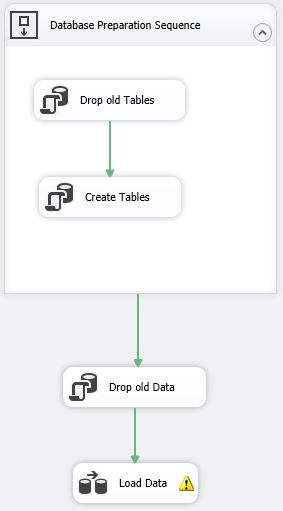
\includegraphics[scale=0.8]{\imageDir/is-control-flow.JPG}
\caption{Integration Service Control Flow}
\label{fig:is-control-flow}
\end{figure}
\ \newline
The following listing describes the components in the control flow:
\begin{itemize}
	\item \emph{Drop old Tables} component drops the existing warehouse tables.
	\item \emph{Create tables} component creates the warehouse tables via an native SQL statement.
	\item \emph{Drop old Data} component drops the old data before data load.
	\item \emph{Load Data} component holds the data flow for data cleanup and restructure.
\end{itemize}
\ \newline
The yellow warn icon is caused by data type changes between the raw data and the prepared data. the data type change is caused by the change of the length of some \emph{nvarchar} typed columns.
\newpage

The image shows the implemented \emph{Data Flow} for the data preparation of the raw data of table \emph{exam} which will be represented by the table \emph{exam} in the warehouse.

\begin{figure}[h]
\centering
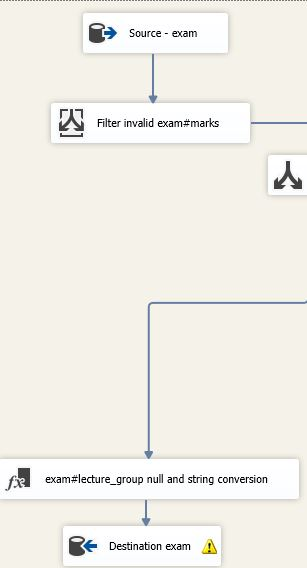
\includegraphics[scale=0.8]{\imageDir/is-data-flow-exam.JPG}
\caption{Integration Service Data Flow for \emph{exam}}
\label{fig:is-data-flow-exam}
\end{figure}
\ \newline
The following listing describes the used \emph{Data Flow} components for data preparation of the table \emph{exam}.
\begin{itemize}
	\item \emph{Source - exam} is a source component and connects to the table \emph{exam} of the raw data.
	\item \emph{Filter invalid exam\# marks} is the \emph{Conditional Split} component which filters the data for valid and invalid marks.
	\item \emph{exam\# lecture\_group null and string conversion} is the \emph{Derived Column} component which transforms the following transformations
	\begin{itemize}
		\item Create the new column \emph{lecture\_group\_str} on stream of type \emph{DT\_WSTR, 10)}
		\item Set the value by the following expression 
		\newline
		$!ISNULL(lecture\_group) ? (''Group '' + (DT\_WSTR,10)lecture\_group) : ''unknown''$
	\end{itemize}
	\item \emph{Destination exam} is the \emph{OLE DB Destination} component which stores the prepared raw data in the destination table \emph{exam}.
\end{itemize}
\ \newline
The yellow warn icon is caused the change of the data type of the column \emph{student\_sex} from \emph{nvarchar(2)} to \emph{nchar(1)}
\newpage

The image shows the implemented \emph{Data Flow} for the data preparation of the raw data of table \emph{lehrer\_prod} which will be represented by the table \emph{teacher} in the warehouse.

\begin{figure}[h]
\centering
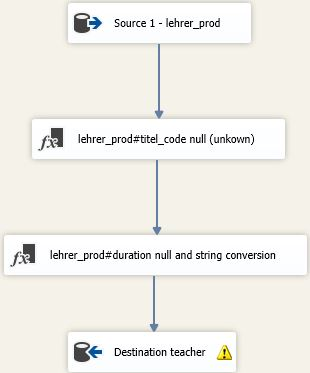
\includegraphics[scale=0.8]{\imageDir/is-data-flow-teacher.JPG}
\caption{Integration Service Data Flow for \emph{lehrer\_prod}}
\label{fig:is-data-flow-teacher}
\end{figure}
\ \newline
The following listing describes the used \emph{Data Flow} components for data preparation of the table \emph{teacher}.
\begin{itemize}
	\item \emph{Source - lehrer\_prod} is a source component and connects to the table \emph{lehrer\_prod} of the raw data.
	\item \emph{lehrer\_prod\# duration null and string conversion} is the \emph{Derived Column} component which transforms the following transformations
	\begin{itemize}
		\item Create the new column \emph{duration\_str} on stream of type \emph{DT\_WSTR, 10)}
		\item Set the value by the following expression 
		\newline
		$!ISNULL(duration) ? ''Duration '' + (DT\_WSTR,10)duration : ''unknown''$
	\end{itemize}
	\item \emph{Destination teacher} is the \emph{OLE DB Destination} component which stores the prepared raw data in the destination table \emph{teacher}.
\end{itemize}
\ \newline
The yellow warn icon is caused the change of the data type of the column \emph{sex} from \emph{nvarchar(255)} to \emph{nchar(1)}

\newpage

The image shows the implemented \emph{Data Flow} for the data preparation of the raw data of table \emph{teacher\_group} which will be represented by the table \emph{teacher\_group} in the warehouse.

\begin{figure}[h]
\centering
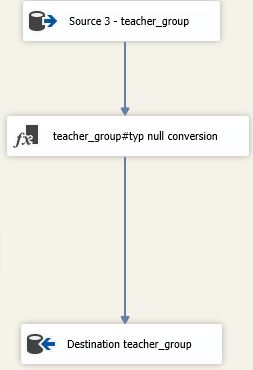
\includegraphics[scale=0.8]{\imageDir/is-data-flow-teacher-group.JPG}
\caption{Integration Service Data Flow for \emph{teacher\_group}}
\label{fig:is-data-flow-teacher}
\end{figure}
\ \newline
The following listing describes the used \emph{Data Flow} components for data preparation of the table \emph{teacher\_group}.
\begin{itemize}
	\item \emph{Source - teacher\_group} is a source component and connects to the table \emph{teacher\_group} of the raw data.
	\item \emph{teacher\_group\# typ null conversion} is the \emph{Derived Column} component which transforms the following transformations
	\begin{itemize}
		\item Set the value by the following expression 
		\newline
		$REPLACENULL(typ,''unknown'')$
	\end{itemize}
	\item \emph{Destination teacher\_group} is the \emph{OLE DB Destination} component which stores the prepared raw data in the destination table \emph{teacher\_group}.
\end{itemize}
\ \newline
This tables holds no null values and therefore are no other transformation necessary.

\newpage

The image shows the implemented \emph{Data Flow} for the data preparation of the raw data of table \emph{student\_group} which will be represented by the table \emph{student\_group} in the warehouse.

\begin{figure}[h]
\centering
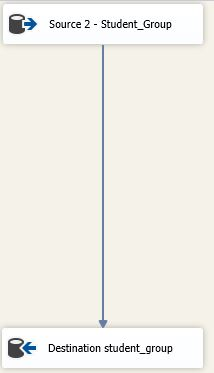
\includegraphics[scale=0.8]{\imageDir/is-data-flow-student-group.JPG}
\caption{Integration Service Data Flow for \emph{student\_group}}
\label{fig:is-data-flow-teacher}
\end{figure}
\ \newline
The following listing describes the used \emph{Data Flow} components for data preparation of the table \emph{student\_group}.
\begin{itemize}
	\item \emph{Source - student\_group} is a source component and connects to the table \emph{student\_group} of the raw data.
	\item \emph{Destination student\_group} is the \emph{OLE DB Destination} component which stores the prepared raw data in the destination table \emph{student\_group}.
\end{itemize}
\ \newline
This table doesn't require any transformation of the data.

\newpage

\section{Analysis Services}
This section deals with the \emph{SSAS Analysis Services} part of the hands on.

\end{document}
